\documentclass{amsart}
\usepackage{amssymb}
\usepackage{amsmath}
\usepackage{tikz,tikz-cd}
\usetikzlibrary{math}
\usetikzlibrary{snakes}
\usepackage{color}
\usepackage[colorlinks=true, citecolor=blue, filecolor=black, linkcolor=black, urlcolor=black]{hyperref}
\usepackage{tcolorbox}

\begin{document}

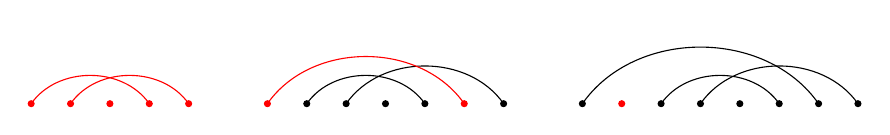
\begin{tikzpicture}[scale = 0.5]
      \tikzset{enclosed/.style={draw, circle, inner sep=0pt, minimum size=.1cm, fill=black}}


    \draw [fill,red] (0,0) circle [radius=0.075] ;
    \draw [fill,red] (1,0) circle [radius=0.075] ;
    \draw [fill,red] (2,0) circle [radius=0.075] ;
    \draw [fill,red] (3,0) circle [radius=0.075] ;
    \draw [fill,red] (4,0) circle [radius=0.075] ;
    \draw [red] (0,0) to [out=55,in=125] (3,0);
    \draw [red] (1,0) to [out=55,in=125] (4,0);


    \draw [fill,red] (6,0) circle [radius=0.075] ;
    \draw [fill] (7,0) circle [radius=0.075] ;
    \draw [fill] (8,0) circle [radius=0.075] ;
    \draw [fill] (9,0) circle [radius=0.075] ;
    \draw [fill] (10,0) circle [radius=0.075] ;
    \draw [fill,red] (11,0) circle [radius=0.075] ;
    \draw [fill] (12,0) circle [radius=0.075] ;
    \draw [] (7,0) to [out=55,in=125] (10,0);
    \draw [] (8,0) to [out=55,in=125] (12,0);
    \draw [red] (6,0) to [out=55,in=125] (11,0);


    \draw [fill] (14,0) circle [radius=0.075] ;
    \draw [fill,red] (15,0) circle [radius=0.075] ;
    \draw [fill] (16,0) circle [radius=0.075] ;
    \draw [fill] (17,0) circle [radius=0.075] ;
    \draw [fill] (18,0) circle [radius=0.075] ;
    \draw [fill] (19,0) circle [radius=0.075] ;
    \draw [fill] (20,0) circle [radius=0.075] ;
    \draw [fill] (21,0) circle [radius=0.075] ;
    \draw [] (16,0) to [out=55,in=125] (19,0);
    \draw [] (17,0) to [out=55,in=125] (21,0);
    \draw [] (14,0) to [out=55,in=125] (20,0);


\end{tikzpicture}

\end{document}